\chapter{Variables, Expresiones y Sentencias}

Una de las más poderosas características de un lenguaje de programación
es la habilidad para manipular {\bf variables}. En términos generales, 
una variable es el nombre que hace referencia a un valor. Podría ser 
más preciso decir que una variable es un contenedor  
que tiene un nombre y que almacena un valor.
\index{variable}


\section{Sentencias de Asignación}
\label{variables}
\index{assignment!statement}
\index{statement!assignment}
\index{$=$ assignment operator}
\index{operator!assignment}


Una {\bf sentencia de asignación} usa el signo de igualdad {\tt =}
y le da un valor a una variable, pero, antes de que asignes un valor 
a una variable, debes primero crear la variable a través de una
declaración (si todavía no existe):
\begin{verbatim}
> my $mensaje;          # declración de una variable, aún sin valor
> $mensaje = 'And now for something completely different';
And now for something completely different
> my $número = 42;      # declaracion de una variable y asignación
42
> $número = 17;         # nueva asignación
17
> my $phi = 1.618033988;
1.618033988
>
\end{verbatim}
%
\index{assignment}
\index{statement!assignment}
\index{declaration!variable}
\index{variable!declaration}

Este ejemplos hace cuatros asignaciones. La primera asigna una cadena de texto
a una nueva variable llamada {\tt \$mensaje}, la segunda asigna 
el número entero {\tt 42} a {\tt \$número}, el tercero reasigna el entero {\tt 17} a
{\tt \$número}, y el cuarto asigna el valor aproximado del número áureo a {\tt \$phi}.

Aquí hay dos características sintácticas importantes que debes entender.

Primero, en Perl, los nombres de las variables comienzan un 
símbolo conocido como un {\emph sigilo}, i.e., un carácter no alfanumérico
como \verb'$', \verb'@', \verb'%', \verb'&', y otros más. Este carácter
especial nos dice y al compilador de Perl (el programa que lee
el código de nuestro programa y lo transfoma en instrucciones 
de computadoras) el tipo de variable que es. Por ejemplo, el 
carácter \$ indica que las variables más arriba son todas variables
escalares, lo cual significa que ellas pueden almacenar un solo valor
en cualquier momento. Veremos más adelante otros tipos de variables las
cuales pueden contener más de un solo valor.
\index{sigil}
\index{scalar}
\index{variable!scalar}
\index{scalar}

Segundo, nota como las tres variables más arriba son 
introducidas con la palabra clave {\tt my}, que es una manera
de declarar una variable nueva. Cuando tu creas una variable nueva
en Perl, necesitas \emph{declararla}, i.e., le deja saber a Perl
que vas a usar una variable nueva; esto se hace comúnmente con la
palabra clave {\tt my}, la cual declara una variable \emph{lexical}.
Explicaremos luego lo que es una variable lexical pero por ahora,
digamos que te permite crear una variable local a una parte 
limitada de tu código. Una de las buenas consecuencias del requerimiento
de declarar variables antes de que las uses es que, si tu cometes
un error al escribir el nombre de una variable, el compilador 
usualmente será capaz de decirte que estás usando una variable que
no ha sido declarada y como resultado te ayudará a encontrar tu error. 
Esto tiene grandes complicaciones las cuales examinaremos más tarde.
\index{my}
\index{declaring variables}
\index{variable!declaration}
\index{lexical}
\index{variable!lexical}

Cuando escribimos al inicio de esta sección que una variable debe
ser declarada antes de ser usada (o solo cuando se usa), esto
significa que la declaración tiene que ser antes (o al punto de) 
del primer uso de la variable en el archivo de texto que contiene el 
programa. Veremos más adelante que los programas no son ejecutados
necesariamente de arriba hacia abajo en el orden en el que las líneas
o código aparecen en el programa; aún así, la declaración de la variable
debe ser antes de su uso en el archivo de texto que contiene el programa.

Si olvidas declara una variable, obtienes un erro sintáctico:
\index{syntax error}

\begin{verbatim}
> $número = 5;
===SORRY!=== Error while compiling <unknown file>
Variable '$número' is not declared
at <unknown file>:1
------> <BOL><HERE>$número = 5;
>
\end{verbatim}
%
Ten presente que podrías obtener diferentes mensajes de
error dependiendo de la versión de Rakudo que ejecutes.
El mensaje arriba se obtuvo en Febrero 2016;
con una versión más nueva (Octubre 2016), el mismo error
se muestra en una forma algo más organizada:
\begin{verbatim}
>
> $número = 5;
===SORRY!=== Error while compiling:
Variable '$número' is not declared
at line 2
------> <BOL><HERE>$número = 5;
>
\end{verbatim}

\index{state diagram}
\index{diagram!state}

Una manera común de representar variables en papel es escribir el 
nombre con una flecha apuntando a su valor. Este tipo de dibujo se le conoce
como un {\bf diagrama de estado} porque muestra en qué estado cada una de las variables
se encuentra (imagínalo como el estado mental de la variable).
La figura\ref{fig.state2} muestra el resultado del ejemplo anterior.

\begin{figure}
\centerline
{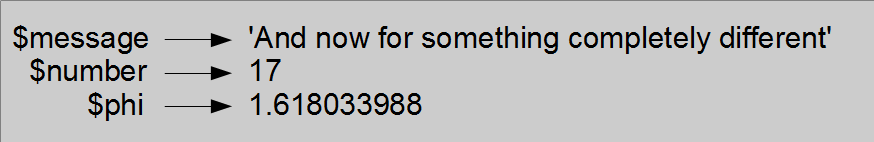
\includegraphics[scale=0.6]{figs/test_5.png}}
\caption{Diagrama de estado.}
\label{fig.state2}
\end{figure}



\section{Nombres de las Variables}
\index{variable}

Los programadores generalmente eligen nombres significativos
para sus variables---ellos documentan el uso de la variable.

Los nombres de las variables pueden ser tan largos como tu desees.
Ellos pueden contener letras y números, pero las variables
definidas por el usuario no pueden comenzar con un número. Los nombres de las
variables son sensibles al uso de mayúsculas y minúsculas, 
i.e., {\tt \$mensaje} no es la misma variable que {\tt \$Mensaje} 
o {\tt \$MENSAJE}. Es legal usar letras mayúsculas, pero es convencional
usar solo letras minúsculas para la mayoría de los nombres de las
variables. No obstante, algunas personas prefieren usar {\tt \$TipoTítulo}
para los nombres de sus variables o hasta {\tt \$MAYÚSCULAS} 
para algunas variables especiales.
\index{lower case}
\index{upper case}
\index{title case}
\index{case!lower}
\index{case!upper}
\index{case!title}


\index{Unicode}
\index{ASCII}
A diferencia de muchos otros lenguajes de programación, Perl~6 
no requiere que las letras y dígitos en los nombres de las variables
sean únicamente ASCII. Puedes usar cualquier tipo de letras Unicode, i.e.
letras de cualquier otro lenguaje en el mundo, así que, por ejemplo,
{\tt \$brücke}, {\tt \$payé} or {\tt \$niño} son nombres de variables
válidos, los cuales pueden ser usados por programadores que hablan 
otros idiomas diferentes al inglés (siempre y cuando estos caracteres
Unicode sean correctamente manipulados por tu editor de texto y tu
configuración de pantalla). De la misma manera, en vez de usar 
\verb"$phi" para el nombre de la variable del número aúreo,
podríamos haber usado la \emph{letra griega minúscula phi},
\verb'φ' (Unicode code point U+03C6). Igualmente, podríamos
haber usado la \emph{letra griega minúscula pi}, $\pi$, 
para la muy conocida razoń de la circunferencia del círculo
al diámetro:
\index{golden ratio}
\index{Unicode}
\index{phi}
\index{pi}

\begin{verbatim}
> my $φ = (5 ** .5 + 1)/2;       # número aúreo
1.61803398874989
> say 'Variable $φ = ', $φ;
Variable $φ = 1.61803398874989
> my $π = 4 * atan 1; 
3.14159265358979
> # podrías también las constante integrada pi o π:
> say pi
3.14159265358979
\end{verbatim}

El carácter de barra baja, \verb"_", puede aparecer en cualquier
parte del nombre de una variable. Usualmente se usa en nombres con
múltiples palabras, tal como \verb"$tu_nombre" o \verb"$airspeed_of_unladen_swallow". 
\index{underscore character}

Hasta puedes usar guiones para crear lo que se conoce como
``kebab case''\footnote{Porque las variables aparecen estar
atravesadas como las piezas de comida preparadas para un barbacoa.}
y nombrar esas variables \verb"$tu-nombre" or \verb"$airspeed-of-unladen-swallow",
y esto las puede hacer más legibles: un guión \verb'-' es válido en una variable
siempre y cuando sea inmediatamente seguido por un carácter alfanumérico.
Por ejemplo, \verb"$doble-clic" or \verb"$la-niña" son nombres legítimos
de variables. Análogamente, puedes usar un apóstrofo \verb"'" 
(también conocido como comilla simple) entre las letras, así que 
\verb"$isn't" o \verb"$o'brien's-age" son identificadores válidos. 
\index{dash}
\index{apostrophe}
\index{single quote}
\index{quote!single}
\index{kebab case}
\index{case!kebab}


Si les da un nombre ilegal a una variable, consigues 
un error sintáctico:
\index{syntax error}

\begin{verbatim}
> my $76trombones = 'big parade'
===SORRY!=== Error while compiling <unknown file>
Cannot declare a numeric variable
at <unknown file>:1
------> my $76<HERE>trombones = "big parade";
>
> my $more§ = 100000;
===SORRY!=== Error while compiling <unknown file>
Bogus postfix
at <unknown file>:1
------> my $more<HERE>§ = 100000;
(...)
\end{verbatim}
%
{\tt \$76trombones} es ilegal porque comienza con un número.
{\tt \$more§} es ilegal porque contiene un carácter ilegal, {\tt
§}. 

Si alguna vez has usado otro lenguaje de programación y 
te has tropezado con un mensaje terso tal como {\tt"SyntaxError: invalid syntax"},
notarás que los diseñadores de Perl han hecho un gran esfuerzo
para proveerte con mensajes de error que sean detallados, útiles
y significativos.
\index{error message}

Muchos lenguajes de programación tienen \emph{palabras claves} o
\emph{palabras reservadas} que son parte de la sintaxis, tales como
{\tt if}, {\tt while}, o {\tt for}, y por lo tanto no pueden ser usadas
para identificar variables porque eso crearía ambigüedad. Dicho problema
no existe en Perl: dado que los nombres de las variables comienzan un sigilo,
el compilador es siempre capaz de diferenciar entre una palabra clave
y una variable. Nombres tales como {\tt \$if} o {\tt \$while} son
sintácticamente identificadores válidos de variables en Perl 
(si estos nombres hacen sentido es un asunto diferente).
\index{sigil}
\index{keyword}
\index{reserved word}


\section{Expresiones y Sentencias}
\label{expr_and_statements}

Una {\bf expresión} es una combinación de términos y operadores.
Los términos pueden ser variables o literales, i.e., valores constantes tales
como un número o una cadena de texto. Al igual que un valor, una variable
es también considerada una expresión. Así que todo lo siguiente
son expresiones legales:
\index{expression}
\index{term}
\index{literal}

\begin{verbatim}
> 42
42
> my $n = 17;
17
> $n;
17
> $n + 25;
42
>
\end{verbatim}
%
Cuando escribes una expresión en el prompt, el interpretador
la {\bf evalúa}, lo que significa que encuentra el valor de la expresión.
En esre ejemplo, {\tt \$n} tiene el valor 17 y {\tt \$n + 25} tiene
el valor 42.
\index{evaluate}

Una {\bf sentencia} es unidad de código que tiene un efecto, 
tal como crear una variable or mostrar un valor, y usualmente
necesita terminar con un punto y coma {\tt ;} (aunque el punto y coma
puede algunas veces ser omitido como veremos más adelante):
\index{statement}
\index{semi-colon}

\begin{verbatim}
> my $n = 17;
17
> say $n;
17
\end{verbatim}
%

La primera línea es una sentencia de asignación que asigna un 
valor a {\tt \$n}. La segunda línea es una sentencia de impresión 
que muestra el valor de {\tt \$n}.

Cuando escribes una sentencia y después presiona {\tt Enter},
el interpretador la {\bf ejecuta}, lo que significa que hace 
lo que la sentencia dicta.
\index{execute}

Una sentencia puede ser combinada con expresiones usando los operadores
aritméticos. Por ejemplo, podrías escribir:
\index{operator}

\begin{verbatim}
> my $respuesta = 17 + 25;
42
> say $respuesta;
42
\end{verbatim}
%

El símbolo \verb'+' es obviamente el operador de adición y,
después de la sentencia de asignación, la variable \verb'$respuesta'
contiene el resultado de la adición. Los términos en cada lado del operador
(aquí 17 y 25) son usualmente llamados los \emph{operadores}
de la operación (una adición en este caso).
\index{operand}
\index{addition operator}
\index{assignment}

Nota que el REPL actualmente muestra el resultado de la asignación
(la primera línea con ``42``), así que la sentencia de impresión 
no era realmente necesaria en este ejemplo \emph{en el REPL};
desde aquí en adelante, para ser breve, generalmente omitiremos las sentencias
de impresión en los ejemplos donde el REPL muestra los resultados.
\index{REPL}

En algunos casos, puedes querer añadir algo a una variable y 
asignar el resultado a la misma variable. Esto se puede escribir
así:

\begin{verbatim}
> my $respuesta = 17;
17
> $respuesta = $respuesta + 25;
42
\end{verbatim}
%

Aquí, \verb"$respuesta" es primero declarada con un valor de 17. La siguiente sentencia
asigna a  \verb"$respuesta" el valor actual de  \verb"$respuesta" (i.e., 17) + 25.
Esta operación es tan común en Perl, como en otro lenguajes de programación, que tiene
un atajo:

\begin{verbatim}
> my $respuesta = 17;
17
> $respuesta += 25;
42
\end{verbatim}
%

\index{$+=$ augmented assignment operator}
El operador \verb"+=" combina el operador de la adición aritmética 
y el operador de asignación para modificar un valor y aplicar 
el resultado a una variable en un solo paso, así que 
\verb"$n += 2" quiere decir: toma el valor actual de \verb|$n|, agrega
2, y asigna el resultado a \verb|$n|. Esta sintaxis funciona con todos
los operadores aritméticos. Por ejemplo, \verb|-=| realiza una
sustracción y una asignación, \verb|*=| una multiplicación y una asignación, etc.
Además de los operadores aritméticos, también puede ser usado con otros operadores 
tal como el operador de la concatenación de cadena de texto que veremos
más adelante.

Agregar 1 a una variable es una versión muy común de esto, 
y como resultado, existe un atajo, el operador de \emph{incremento},
el cual incrementa su argumento por uno, y devuelve el valor incrementado: 
\index{increment operator}
\index{++ increment operator}
\index{operator!++ (increment)}

\begin{verbatim}
> my $n = 17;
17
> ++$n;
18
> say $n;
18
\end{verbatim}
%
Esto se conoce como el operador de incremento prefijo, porque el operador \verb|++|
se coloca antes que la variable a ser incrementada. También hay una versión sufijo (posfijo),
\verb|$n++|, la cual devuelve el valor actual y después incrementa la variable por uno. 
No haría ninguna diferencia en el fragmento de código más arriba, pero el resultado puede
ser diferente en expresiones un poco más complejas.

También hay un operador de decremento \verb|--|, el cual disminuye 
su argumento por uno y existe en la forma prefijo y posfijo. 
\index{decrement operator}
\index{\verb'--' decrement operator}
\index{operator!$--$ (decrement)}



\section{Modo Script}

Hasta ahora hemos ejecutado Perl  en el {\bf modo interactivo}, lo que 
significa que tu interactúas directamente con el interpretador (el REPL).
El modo interactivo es una buena manera de comenzar, si estás trabajando 
con más de varias líneas de código, puede ser un poco torpe y hasta tedioso.
\index{interactive mode}

La alternativa es usar un editor de texto y guardar el código en un archivo de 
texto conocido como un {\bf script} y después ejecutar el interpretador en el 
{\bf modo script} para ejecutar el script. Por convención, los scripts de Perl~6 
tienen nombres que terminan con {\tt .pl}, {\tt .p6} o {\tt .pl6}.
\index{script}
\index{script mode}

Aseguráte de usar un \emph{editor de texto} y no un \emph{programa de procesamiento de texto}
(como MS Word, OpenOffice o LibreOffice Writer). Hay un gran número de editores
de texto disponible gratis. En Linux, podrías usar \emph{vi} (o \emph{vim}), 
\emph{emacs}, \emph{gEdit}, o \emph{nano}. En Windows, puedes usar \emph{notepad} (muy limitado),
o \emph{notepad++}. También hay editores multiplataforma o entorno de desarrollo integrado
(IDES por su siglas en inglés) los cuales proveen la funcionalidad de un editor de texto. 
Entre ellos están \emph{padre}, \emph{eclipse}, o \emph{atom}. Muchos de estos proveen 
varias funcionalidades de resaltado de sintaxis, que puede ayudarte a usar 
la sintaxis correcta (y encontrar algunos errores sintácticos).
\index{syntax!highlighting}
\index{text editor!emacs}
\index{text editor!vi}
\index{text editor!vim}
\index{text editor!gEdit}
\index{text editor!padre}
\index{text editor!eclipse}
\index{text editor!nano}
\index{text editor!notepad++}
\index{text editor!atom}

Una vez que has guardado tu código en un archivo de texto (por ejemplo,
\verb|mi_script.pl6|), puedes ejecutar el programa mediante el siguiente
comando en el prompt del sistema operativo (por ejemplo en una consola de 
Linux or en una ventana \verb|cmd| en Windows):
\begin{verbatim}
perl6 mi_script.pl6
\end{verbatim}

Dado que Perl provee ambos modos, 
puedes ejecutar piezas de código en el modo interactivo 
antes que las pongas en un script. Pero existen diferencias entre 
el modo interactivo y el modo script que pueden confundir.
\index{interactive mode}
\index{script mode}

Por ejemplo, si estás usando el interpretador de Perl~6 como una
calculadora, podrías escribir:

\begin{verbatim}
> my $millas = 26.2;
26.2
> $millas * 1.61;
42.182
\end{verbatim}

La primera línea asigna un valor a {\tt \$millas} y muestra ese valor.
La segunda línea es una expresión, así que el interpretador la evalúa
y muestra el resultado. Resulta que un maratón es alrededor de 42~kilómetros.

Pero si escribe el mismo código en un script y lo ejecuta, no obtienes
ningún resultado. En el modo script, una expresión por sí misma no tiene
ningún efecto visible. Perl actualmente evalúa la expresión, pero no muestra
el valor a menos que se lo indiques:

\begin{verbatim}
my $millas = 26.2;
say $millas * 1.61;
\end{verbatim}

Este comportamiento puede ser confuso al principio. Examinemos
el por qué.

Un script usualmente contiene una secuencia de sentencias. Si hay más 
de una sentencia, los resultados aparecen uno por uno al 
tiempo que las sentencias de impresión se ejecutan.

Por ejemplo, considera el siguiente script:

\begin{verbatim}
say 1;
my $x = 2;
say $x;
\end{verbatim}
%
Produce el siguiente resultado:

\begin{verbatim}
1
2
\end{verbatim}
%
La sentencia de asignación no produce ningún resultado.

Para comprobar tu entendimiento, escribe las siguientes sentencias
en el interpretador de Perl y observa lo que hacen:

\begin{verbatim}
5;
my $x = 5;
$x + 1;
\end{verbatim}

Ahora pon la mismas sentencias en un script y ejecútalo. 
Cuál es el resultado? Transformar cada expresión en una sentencia 
de impresión y después ejecuta el script modificado otra vez.

\section{Modo de una sola línea}

Perl también tiene un \emph{modo de una sola línea} (modo one-liner), el cual te permite 
escribir un script bien corto directamente en el prompt del sistema
operativo. Debido a esto, dicho scripts son conocidos como one-liners.
 En Windows, podría lucir de la siguiente manera:
\index{one-liner mode}
\label{one-liner mode}

\begin{verbatim}
C:\Users\Laurent>perl6 -e "my $valor = 42; say 'La respuesta es ', $valor;"
La respuesta es 42

\end{verbatim}

La opción {\tt -e} le dice al compilador que el script
a ser ejecutado no está guardado en un archivo de texto sino
que en cambio está escrito en el prompt entre comillas inglesas
inmediatamente después de dicha opción.

En Unix y Linux, reemplazarías las comillas inglesas con apóstrofos
(o comillas simples)  y los apóstrofos con comillas inglesas:
\index{apostrophe}
\index{quote mark}

\begin{verbatim}
$  perl6 -e 'my $valor = 42; say "La respuesta es $value";'
La respuesta es 42

\end{verbatim}

El one-liner más arriba puede no parecer útil, pero 
one-liners desechables pueden ser muy prácticos para realizar
operaciones simples, tal como modificar un archivo que no
está formateado apropiadamente, sin tener que guardar un script
en archivo separado antes de ejecutarlo.  

No daremos ningunos detalles adicionales sobre el modo 
de una sola línea, pero daremos más ejemplos útiles más
adelante en este libro; por ejemplo,
Subsección~\ref{one-liner-example},
Subsección~\ref{rot13_oneliner} (resolviendo el ejercicio ``rot-13''), o
Subsección~\ref{sol_cartalk} (resolviendo el ejercicio sobre 
letras dobles consecutivas). 



\section{Orden de Operaciones}
\index{order of operations}
\index{PEMDAS}
\index{operator precedence}
\index{precedence!operator}

Cuando una expresión contiene más de un operador, el orden 
de evaluación depende en el {\bf orden de operaciones} o 
la \emph{precedencia de operadores}. Para los operadores matemáticos,
Perl sigue la convención matemática. El acrónimo {\bf PEMDAS}\footnote{Los estudiantes 
estadounidenses se les enseña a usar el mnemónico 
"Please Excuse My Dear Aunt Sally" para recordar el orden 
correcto de las letras en el acrónimo.} es una manera muy útil de recordar
las reglas\footnote{En español, podrías utilizar "Por Favor Excusa Mi Dragón Azul Sancho" para
recordar el orden correcto.}:
 
\begin{itemize}

\item {\bf P}aréntesis tienen la mayor precedencia y pueden ser 
usado para forzar una expresión a evaluar en el orden que deseas.
Dado que las expresiones en paréntesis son evaluadas primero, 
{\tt 2 * (3-1)} es 4, y {\tt (1+1)**(5-2)} es 8.  También puedes usar 
paréntesis para hacer una expresión más legible, como en {\tt (\$minuto * 100) / 60},
aunque no cambia el resultado.
\index{$()$ parenthesis operator}

\item {\bf E}xponente (potenciación) es la siguiente en el nivel de precedencia, así
que {\tt 1 + 2**3} es 9 (1 + 8), no 27, y {\tt 2 * 3**2} es 18, no 36.
\index{$**$ exponentiation operator}
\index{operator!$**$ (exponentiation)}

\item {\bf M}ultiplicación y {\bf D}ivisión tiene mayor precedencia
  que {\bf A}dición y {\bf S}ustracción.  Por lo tanto, {\tt 2*3-1} es 5, no
  4, y {\tt 6+4/2} es 8, no 5.
\index{$*$ multiplication operator}
\index{operator!$*$ (multiplication)}
\index{$/$ division operator}
\index{operator!$/$ (division)}

\item Operadores con la misma precedencia son usualmente evaluados
de izquierda a derecha (excepto la potenciación). Así que en la expresión
{\tt \$grados / 2 * pi}, la división ocurre primero y el resultado 
es multiplicado por {\tt pi}, el cual no es el resultado esperado. (Nota que 
{\tt pi} no es una variable, pero una constante predefinida en Perl~6, y por lo tanto
no requiere un sigilo.) Para dividir por $2 \pi$, puedes usar paréntesis: 
\index{sigil}
\index{pi}
  
\begin{verbatim}
my $result = $degrees / (2 * pi);  
\end{verbatim}  
 
o escribir 
  {\tt \$grados / 2 / pi} o {\tt \$grados / 2 / $\pi$}, lo cual
  divide \verb'$grados' por 2, y después divide el resultado de esa
  operación por $\pi$ (el cual es equivalente a \verb'$grados'
  dividido por $2 \pi$).

\end{itemize}

Yo trato de no recordar la precedencia de los operadores. Si no puedo 
determinar la precedencia al mirar la expresión, uso paréntesis para
hacerlo obvio. Si no sé cuál de dos operadores tiene la mayor precedencia, entonces 
la siguiente persona manteniendo mi código podría tampoco saberlo.
\index{precedence}
\index{parentheses}


\section{Operaciones de Cadena de Texto}
\label{string_operations}
\index{string!operation}
\index{operator!string}
\index{coercion}
\index{type!coercion}

En general, no puedes realizar operaciones matemáticas con cadenas de texto,
a menos que las cadenas de texto se parezcan tanto a los números que 
Perl las transforma o \emph{coacciona} en números y todavía hace sentido.
Así que los siguientes casos son ilegales:

\begin{verbatim}
'2'-'1a'    'eggs'/'easy'    'third'*'a charm'
\end{verbatim}
%

Por ejemplo, esto produce un error:

\begin{verbatim}
> '2'-'1a'
Cannot convert string to number: trailing characters after number 
in '1?a' (indicated by ?)
  in block <unit> at <unknown file>:1
\end{verbatim}
%

Pero la siguiente expresiones son válidas porque estas cadenas de texto
pueden ser coaccionadas en números sin ninguna ambigüedad:
\begin{verbatim}
> '2'-'1'
1
> '3'/'4'
0.75
\end{verbatim}
%

El operador \verb'~' realiza la {\bf concatenación de cadenas de texto}, 
lo cual quiere decir que une las cadenas de texto al enlazarlas de
extremo a extremo. Por ejemplo:
\index{string concatenation}
\index{string!concatenation}

\begin{verbatim}
> my $primera = 'hidro'
throat
> my $segunda = 'avión'
warbler
> $primera ~ $segunda
hidroavión
\end{verbatim}
%
El operador {\tt x} también funciona con cadenas de texto; básicamente
realiza repeticiones. Por ejemplo:
\index{string repetition}

\begin{verbatim}
> 'ab' x 3;
ababab
> 42 x 3
424242
> 3 x 42
333333333333333333333333333333333333333333
\end{verbatim}

Nota que, aunque el operador {\tt x} se parece al operador
de multiplicación que escribimos a mano, {\tt x} obviamente 
no es conmutativo, contrario al operador de multiplicación 
{\tt *}. El primer operando es una cadena de texto o es coaccionado
en una (i.e., transformado en una cadena de texto:
{\tt 42} es coaccionado en {\tt '42'})  , y el segundo operando
tiene que ser un número o algo que pueda ser transformado en 
un número.
\index{commutativity}
\index{coercion}


\section{Comentarios}
\index{comment}

A medida que los programas crecen y se vuelven más complicados,
ellos se vuelven menos legible. Los lenguajes formales son denso, y es usualmente
difícil mirar a un fragmento de código y descifrar lo que está haciendo,
o por qué lo está haciendo.

Por esta razón, es muy buena idea agregar notas a tus programas que expliquen en un
lenguaje natural lo que el programa hace. Estas notas son conocidas como {\bf comentarios},
y comienzan con el símbolo \verb|#|:

\begin{verbatim}
# computar el porcentaje de la hora que ha pasado
my $porcentaje = ($minuto * 100) / 60;
\end{verbatim}
%
En este caso, el comentario aparece en una línea por sí mismo. También puedes
colocar comentarios al final de una línea:

\begin{verbatim}
$porcentaje = ($minuto * 100) / 60;     # porcentaje de una hora
\end{verbatim}
%
Todo desde el inicio de {\tt \#} al final de la línea es ignorado---lo que significa
que no tiene un efecto en el ejecución del programa.

Los comentarios son más útiles cuando documentan características del código
que no obvias. Es razonable asumir que el lector puede descifrar lo que 
hace el código; es más útil explicar explicar el {\em por qué}.

Este comentario es redundante con el código e inservible:

\begin{verbatim}
my $valor = 5;        # asignar 5 a $valor
\end{verbatim}
%
Por el contrario, este comentario contiene información útil que no está
presente en el código:

\begin{verbatim}
my $velocidad = 5;     # la velocidad es en metros/segundos. 
\end{verbatim}
%
Nombres de variables que son buenos y adecuados pueden reducir la necesidad 
de comentario, pero nombres muy largos pueden hacer expresiones sean difíciles
de leer, por lo tanto debe existir un balance.
\index{variable name}


\section{Depuración de Programas}
\index{debugging}
\index{bug}

Tres tipos de errores pueden ocurrir en un programa: errores
sintácticos, errores al tiempo de ejecución, y  errores semánticos.
Es muy útil saber distinguirlos para ratrearlos más rápido.

\begin{description}

\item[Error sintáctico] La ``sintaxis'' se refiere a la estructura de un 
programa. Por ejemplo, los paréntesis deben estar en parejas, así que 
{\tt (1 + 2)} es legal mientras {\tt 8)} es un \emph{error sintáctico}.
\footnote{Aquí estamos usando ``error sintáctico'' como un cuasi-sinónimo
para ``error al tiempo de compilación``; ellos no son exactamente la misma cosa
(en teoría, puedes tener errores sintácticos que no son errores al tiempo
de compilación y viceversa), pero se pueden considerar aquí lo mismo por razones
prácticas. En Perl~6, errores al tiempo de compilación tienen la cuerda de texto
``===SORRY!==='' al inicio del mensaje de error.}

\index{error!syntax}
\index{error message}
\index{syntax} 
\index{syntax!error}

Si en tu programa hay un error sintáctico, Perl muestra 
un mensaje de error y abandona la ejecución sin siquiera 
comenzar a ejecutar el programa. Durante las primeras semanas de 
tu carrera de programación, podrías invertir mucho tiempo rastreando
errores sintácticos. A medida que ganas experiencia, cometerás menos errores
y lo encontraras más rápido.


\item[Error al tiempo de ejecución] El segundo tipo de error es un 
error al tiempo de ejecución, llamado así porque el error no aparece hasta que 
el programa ha comenzado a ejecutarse. Estos errores también son conocidos
como \emph{excepciones} porque ellos usualmente indican que algo excepcional (y malo)
ha ocurrido. 
\index{runtime error}
\index{error!runtime}
\index{exception} 
\index{safe language} 
\index{language!safe}

Los errores al tiempo de ejecución son raros en programas simples 
que verás en los primeros capítulos, así que podría pasar un rato antes
que encuentres uno. Ya hemos visto un ejemplo de tales errores, aunque, 
al inicio de la Sección~\ref{string_operations} (p.~\pageref{string_operations}), 
cuando intentamos sustraer \verb"'2'-'1a'".


\item[Error semántico] El tercer tipo de error es \emph{semántico}, lo que
significa que está relacionado con el significado. Si en tu programa hay un error
semántico, el programa se ejecutará sin generar mensajes de error. Específicamente,
hará lo que \emph{dijiste} que hiciera, pero no lo que habías \emph{previsto}.
\index{semantic error}
\index{error!semantic}
\index{error message}

La identificación de errores semánticos pueden ser complicada porque requiere
que trabajes de atrás hacia adelante mediante la observación de la salida
del programa y tratando de descifrar lo que el programa esta haciendo.

\end{description}


\section{Glosario}

\begin{description}

\item[Variable]  Informalmente, un nombre que hace referencia a un valor. En términos
precisos, una variable es un contenedor que tiene un nombre y almacena un valor.
\index{variable}

\item[Asignación]  Un sentencia que asigna un valor a una variable.
\index{assignment}

\item[Diagrama de estado]  Una representación gráfica de un conjunto de variables
y los valores a los que hacen referencia.
\index{state diagram}

\item[Palabra clave]  Una palabra reservada que es usada para parsear
un programa; en muchos lenguajes, no puedes usar palabras claves tales como
{\tt if}, {\tt  for}, y {\tt while} como nombres de variables.
Este problema usualmente no ocurre en Perl porque los nombres de variables
comienzan con un \emph{sigilo}.
\index{keyword}
\index{sigil}

\item[Operando] Un valor o término al lado de un operador que es usado
en su evaluación.
\index{operand}

\item[Término]  Una variable or valor literal.
\index{term}

\item[Expresión]  Una combinación de operadores y términos que 
representan un valor único.
\index{expression}

\item[Evaluar]  Simplificar una expresión al realizar las operaciones 
para obtener un valor único.
\index{evaluate}

\item[Sentencia]  Una sección de código que representa un comando o una acción. Hasta ahora,
las sentencias que hemos visto son las asignaciones y las sentencias de impresión. Las sentencias
usualmente terminan con un punto y coma.
\index{statement}

\item[Ejecutar]  Poner una sentencia en acción y hacer lo que dice.
\index{execute}

\item[Modo interactivo (o modo interpretador):] Una manera de usar el interpretador 
de Perl al escribir código en el prompt.
\index{interactive mode}

\item[Modo script] Una manera de usar el interpretador 
de Perl para leer código desde un script y ejecutarlo.
\index{script mode}

\item[Modo de una sola línea (one-liner)] Una manera de usar el interpretador 
de Perl para leer código pasado al prompt del sistema operativo 
y ejecutarlo.
\index{one-liner mode}

\item[Script] Un programa almacenado en un archivo de texto.
\index{script}

\item[Order de operaciones]  Reglas que dictan el orden en el que las expresiones
que contienen varios operadores y operandos son evaluadas.
También se conoce como precedencia de operadores.
\index{order of operations}
\index{operator precedence}
\index{precedence!operator}

\item[Concatenar]  Unir dos cadenas de texto de extremo a extremo.
\index{concatenation}

\item[Comentario]  Información en una programa que está dirigida a otros programadores
(o cualquier persona leyendo el código fuente) y que no tiene ningún efecto en 
la ejecución del programa.
\index{comment}

\item[Error sintáctico]  Un error en un programa que lo hace imposible
parsear (y por lo tanto imposible de compilar y ejecutar).
\index{syntax!error}

\item[Excepción]  Un error que es detectado mientra que el programa se ejecuta.
\index{exception}

\item[Semántica]  El significado de un programa.
\index{semantics}

\item[Error semántico] Un error en un programa que causa que haga algo 
diferente a lo que programador pretendía hacer.
\index{semantic error}

\end{description}


\section{Ejercicios}

\begin{exercise}

Repeating our advice from the previous chapter, whenever you learn
a new feature, you should try it out in interactive mode (under 
the REPL) and make errors on purpose to see what goes wrong.
\index{interactive mode}
\index{REPL}

\begin{itemize}

\item We've seen that {\tt \$n = 42} is legal.  What about {\tt 42 = \$n}?

\item How about {\tt \$x = \$y = 1}? (Hint: note that you will 
have to declare both variables, for example with a statement 
such as {\tt my \$x; my \$y;} or possibly {\tt my (\$x, \$y);}, 
before you can run the above.)

\item In some languages, statements don't have to end with a semi-colon, 
{\tt ;}. What happens in script mode if you omit a semi-colon at the end
of a Perl statement?
\index{semi-colon}

\item What if you put a period at the end of a statement?

\item In math notation you can multiply $x$ and $y$ like this: $x y$.
What happens if you try that in Perl?

\end{itemize}

\end{exercise}


\begin{exercise}

Practice using the Perl interpreter as a calculator: 
\index{calculator}

\begin{enumerate}

\item The volume of a sphere with radius $r$ is $\frac{4}{3} \pi r^3$.
  What is the volume of a sphere with radius 5?

\item Suppose the cover price of a book is \$24.95, but bookstores get a
  40\% discount.  Shipping costs \$3 for the first copy and 75 cents
  for each additional copy.  What is the total wholesale cost for
  60 copies?

\item If I leave my house at 6:52 a.m. and run 1 mile at an easy pace
  (8:15 per mile), then 3 miles at tempo (7:12 per mile) and 1 mile at
  easy pace again, what time is it when I complete my running exercise?
\index{running pace}

\end{enumerate}
\end{exercise}

